\documentclass[10pt,mathserif]{beamer}

\usepackage{graphicx,amsmath,amssymb,tikz,psfrag}
\usetikzlibrary{calc}
\usepackage{pgfplots}
\include{defs}

%% formatting

\mode<presentation>
\usetheme{default}
\setbeamertemplate{navigation symbols}{}
\usecolortheme[rgb={0.745, 0.117, 0.176}]{structure}
\setbeamertemplate{itemize subitem}{--}
\setbeamertemplate{frametitle} {
	\begin{center}
	  {\large\bf \insertframetitle}
	\end{center}
}

\newcommand\footlineon{
  \setbeamertemplate{footline} {
    \begin{beamercolorbox}[ht=2.5ex,dp=1.125ex,leftskip=.8cm,rightskip=.6cm]{structure}
      \footnotesize \insertsection
      \hfill
      {\insertframenumber}
    \end{beamercolorbox}
    \vskip 0.45cm
  }
}
\footlineon

%\AtBeginSection[] 
%{ 
%	\begin{frame}<beamer> 
%		\frametitle{Outline} 
%		\tableofcontents[currentsection,currentsubsection] 
%	\end{frame} 
%} 

%% begin presentation

\title{\large \bfseries Valbal Trajectory Planning}

\author{Joan Creus-Costa and John Dean\\[3ex]
\small Stanford Student Space Initiative}

\date{\today}

\begin{document}

\frame{
\thispagestyle{empty}
\titlepage
}

\section{ValBal}
\begin{frame}
\frametitle{ValBal}

\begin{itemize}
\item Research project by the Stanford Space Initiative (undergrad student club).
\item High altitude latex balloon platform that controls its altitude by venting lifting gas and dropping ballast mass.
\item Very cheap (sub thousand dollars), long endurance (5 days demonstrated).
\item Potential applications: hurricane data collection, radar probing of Greenland ice, lightning research, data relay\dots
\item Control: in altitude (remain between bounds while minimizing control effort), in space (pick altitude to get good winds).
\end{itemize}
{\scriptsize
\begin{enumerate}
\item A. Sushko, A. Tedjarati, J. Creus-Costa, S. Maldonado, K. Marshland and M. Pavone, ``Low cost, high endurance, altitude-controlled latex balloon for near-space research (ValBal),'' 2017 IEEE Aerospace Conference, Big Sky, MT, 2017, pp. 1-9.
\item A. Sushko et al., ``Advancements in low-cost, long endurance, altitude controlled latex balloons (ValBal),'' 2018 IEEE Aerospace Conference, Big Sky, MT, 2018, pp. 1-10.
\end{enumerate}}
\end{frame}

\begin{frame}

\begin{center}\includegraphics[width=0.4\linewidth,trim={0cm 13cm 0cm 5cm},clip]{render.jpg}\hspace{1cm}\includegraphics[width=0.4\linewidth,trim={12cm 2cm 25cm 12cm},clip]{vbpic.jpg}\end{center}
\end{frame}


\begin{frame}
\centering
\includegraphics[width=0.9\linewidth]{valbal-map.png}
\includegraphics[width=0.6\linewidth]{thegraph.pdf}
%\vfill
\end{frame}

\section{Trajectory Planning}



\section{Altitude Control}
\subsection{System Dynamics}

\begin{frame}
\frametitle{System Dynamics}
\begin{columns}
\column{0.6\textwidth}
\begin{itemize}\itemsep=12pt
\item Assumptions
\vspace*{0.5em}
\begin{itemize}
\item $v_t$ is small
\item $F_d \propto v$ i.e. drag is linear.
\item $F_l - F_g = F_d$ i.e. the balloon is always at terminal velocity 
\end{itemize}
\item Equations of motion
\vspace*{0.5em}
\begin{itemize}
\item let $l = F_l - F_g$ be the net lift on the balloon
\item $\dot l$ is commanded by controller
\item $v = k_{d} \int \dot l \, dt $
\item $h = \int v \, dt$
\item $\mathcal{L}\{\cdot\} = k_{d} / s^2$
\end{itemize}
\end{itemize}

\column{0.4\textwidth}

\begin{center}
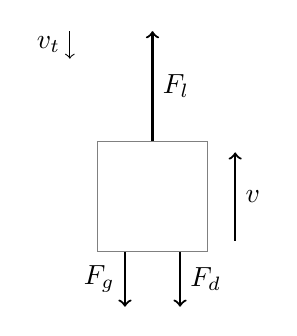
\begin{tikzpicture}[scale=0.7]
    \draw[gray] (-1,-1) rectangle (1,1);
    \draw[thick,->] (0,1) -- (0,3) node[midway,right]{$F_l$};
    \draw[thick,->] (.5,-1) -- (.5,-2) node[midway,right]{$F_d$};
    \draw[thick,->] (-.5,-1) -- (-.5,-2) node[midway,left]{$F_g$};
    \draw[thick,->] (1.5,-0.8) -- (1.5,0.8) node[midway,right]{$v$};
    \draw[->] (-1.5,3) -- (-1.5,2.5) node[midway,left]{$v_t$};
\end{tikzpicture}
\end{center}

$F_d$: Force of drag\\
$F_g$: Gravity\\
$F_l$: Buoyant force\\
$v$: vertical velocity of balloon\\
$v_t$: vertical velocity of surrounding air
\end{columns}
\end{frame}

\begin{frame}
\frametitle{Open Loop Block Diagram}
\begin{center}
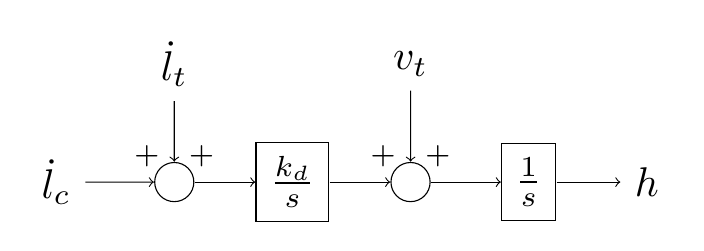
\begin{tikzpicture}[scale=2,
     block/.style = {draw, rectangle,node distance=1cm},
     input/.style = {node distance=1cm},
     output/.style = {node distance=1cm},
     arrow/.style={draw, -latex,node distance=2cm},
     pinstyle/.style = {pin edge={latex-, black,node distance=2cm}},
     sum/.style = {draw, circle, node distance=1cm},
     gain/.style = {regular polygon, regular polygon sides=3,draw, fill=white, text width=1em,
      inner sep=0mm, outer sep=0mm,
      shape border rotate=-90}
    ]
    \begin{scope}[scale=.75, transform shape]
    \node [input] (cinput) {$\dot l_c$};
    \node [sum, right of=cinput] (dlift) {};
    \node [input, above of=dlift] (ldist) {$\dot l_t$};
    \node [block, right of=dlift] (lint) {$\frac{k_d}{s}$};
    \node [sum, right of=lint] (velocity) {};
    \node [input, above of=velocity] (vdist) {$v_t$};
    \node [block, right of=velocity] (vint) {$\frac{1}{s}$};
    \node [output, right of=vint] (h) {$h$};

    \draw[->] (cinput) -- (dlift) node [above left] {\scriptsize +};
    \draw[->] (ldist) -- (dlift) node [above right] {\scriptsize +};
    \draw[->] (dlift) -- (lint);
    \draw[->] (lint) -- (velocity) node [above left] {\scriptsize +};
    \draw[->] (vdist) -- (velocity) node [above right] {\scriptsize +};
    \draw[->] (velocity) -- (vint) node [above right] {};
    \draw[->] (vint) -- (h) node [above right] {};
    \end{scope}
\end{tikzpicture}
\end{center}
\vspace{1cm}
$\dot l_c$: commanded change in lift (valve and ballast actions) \\
$\dot l_t$: atmospheric lift disturbance \\
$v_t$: atmosphereic velocity disturbance \\
$h$: altitude 
\end{frame}



\section{Spaghetti}

\begin{frame}
\frametitle{Spaghetti Controller Motivation}
\begin{itemize}
\item Use a simple linear compensator to stabilize altitude with robust stability margins

\item 
\end{itemize}
\end{frame}

\begin{frame}
\frametitle{Spaghetti Block Diagram}
\begin{center}
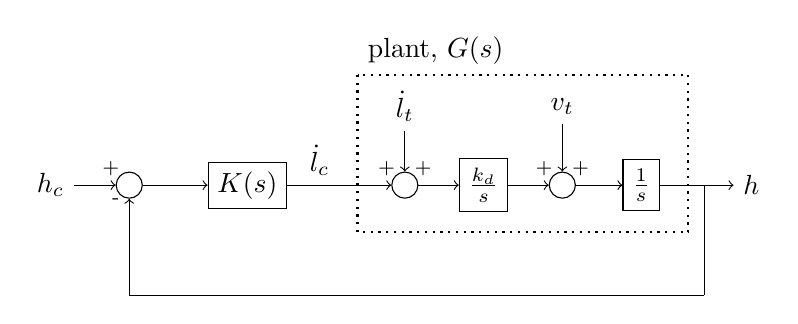
\begin{tikzpicture}[scale=2,
     block/.style = {draw, rectangle,node distance=1cm},
     input/.style = {node distance=1cm},
     output/.style = {node distance=1cm},
     arrow/.style={draw, -latex,node distance=2cm},
     pinstyle/.style = {pin edge={latex-, black,node distance=2cm}},
     sum/.style = {draw, circle, node distance=1cm},
     gain/.style = {regular polygon, regular polygon sides=3,draw, fill=white, text width=1em,
      inner sep=0mm, outer sep=0mm,
      shape border rotate=-90}
    ]
        
    \node [input] (hcmd) {$h_c$};
    \node [sum,right of=hcmd] (hsum) {};    
    \node [block,right of=hsum, node distance=1.5cm] (lead) {$K(s)$};
    \node [sum, right of=lead, node distance=2cm] (dlift) {};
    \node [input, above of=dlift] (ldist) {$\dot l_t$};
    \node [block, right of=dlift] (lint) {$\frac{k_d}{s}$};
    \node [sum, right of=lint] (velocity) {};
    \node [input, above of=velocity] (vdist) {$v_t$};
    \node [block, right of=velocity] (vint) {$\frac{1}{s}$};
    \node [output, right of=vint,node distance=1.4cm] (h) {$h$};

    \draw[->] (hcmd) -- (hsum) node [above left] {\scriptsize +};
    \draw[->] (hsum) -- (lead);
    \draw[->] (lead) -- node [above left] {$\dot l_c$} (dlift)  node [above left] {\scriptsize +};
    \draw[->] (ldist) -- (dlift) node [above right] {\scriptsize +};
    \draw[->] (dlift) -- (lint);
    \draw[->] (lint) -- (velocity) node [above left] {\scriptsize +};
    \draw[->] (vdist) -- (velocity) node [above right] {\scriptsize +};
    \draw[->] (velocity) -- (vint) node [above right] {};
    \draw[->] (vint) -- (h) node [above right] {};
    \draw  (h) ++ (-.3,0) -- ++(0,-.7) coordinate (fb);
    \draw[->] (fb) -| (hsum) node [below left] {\scriptsize -};
    \draw[thick,dotted] ($(dlift)+(-.3cm,.7cm)$) node [above right] {plant, $G(s)$} rectangle ($(vint)+(.3cm,-.3cm)$) ;

\end{tikzpicture}
\end{center}
\vspace{1cm}
$K(s)$: First order lead compensator.
\end{frame}

\begin{frame}{Spaghetti Flight}
\begin{center}

\includegraphics[width=1\linewidth,trim={10 0 10 0cm},clip]{flight.png}
\begin{itemize}
\item 120hr flight from December with spaghetti as controller 
\begin{itemize}
\item blue shows ballast events, green shows vent events
\item temperature shows sunset/sunrise, large effect on ballast use
\end{itemize}
\item issues durring flight:
\begin{itemize}
\item valve controller had software bug, instead of changing duty cylce, one threshold met valve was repeatedly opened
\item At end of flight, balloon has low overpressure--opening valve has no effect until balloon rises high enough
\end{itemize}
\end{itemize}
\end{center}
\end{frame}


\begin{frame}{Oscillations}

\includegraphics[width=1\linewidth,trim={10 0 10 0cm},clip]{osc.png}
\end{frame}

\begin{frame}{Velocity Estimator}

Lowpass filtered velocity estimate that fuses information on actions from the controller.
\begin{center}
\includegraphics[width=.8\linewidth,trim={10 0 10 0cm},clip]{est.png}
\end{center}
\vspace{-0.5cm}
\[ \mathcal{L}\{ \hat v \} = H_1(s) \mathcal{L}\{h\} + H_2(s) \mathcal{L} \{\dot l_c\} \]
$H_1(s)$ is differentiation and 2nd order lowpass filter\\
$H_2(s)$ is integration with decay (estimate of effect of actions, decays to 0 over time)
\end{frame}


\section{Lasagna}

\begin{frame}
\frametitle{Lasagna Block Diagram}
\vspace{-1cm}
\begin{center}
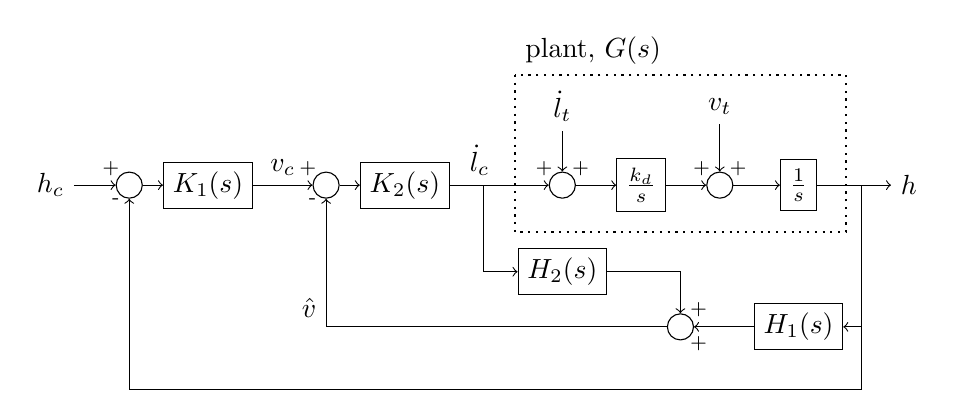
\begin{tikzpicture}[scale=2,
     block/.style = {draw, rectangle,node distance=1cm},
     input/.style = {node distance=1cm},
     output/.style = {node distance=1cm},
     arrow/.style={draw, -latex,node distance=2cm},
     pinstyle/.style = {pin edge={latex-, black,node distance=2cm}},
     sum/.style = {draw, circle, node distance=1cm},
     gain/.style = {regular polygon, regular polygon sides=3,draw, fill=white, text width=1em,
      inner sep=0mm, outer sep=0mm,
      shape border rotate=-90}
    ]
        
    \node [input] (hcmd) {$h_c$};
    \node [sum,right of=hcmd] (hsum) {};    
    \node [block,right of=hsum, node distance=1cm] (K1) {$K_1(s)$};
    \node [sum,right of=K1, node distance=1.5cm] (vsum) {};
    \node [block, right of=vsum] (K2) {$K_2(s)$};
    \node [sum, right of=K2, node distance=2cm] (dlift) {};
    \node [input, above of=dlift] (ldist) {$\dot l_t$};
    \node [block, right of=dlift] (lint) {$\frac{k_d}{s}$};
    \node [sum, right of=lint] (velocity) {};
    \node [input, above of=velocity] (vdist) {$v_t$};
    \node [block, right of=velocity] (vint) {$\frac{1}{s}$};
    \node [output, right of=vint,node distance=1.4cm] (h) {$h$};
    \node [block, below of=vint,node distance=1.8cm] (H1) {$H_1(s)$};
    \node [block, below of=dlift,node distance=1.1cm] (H2) {$H_2(s)$};
    \node [sum, left of=H1,node distance=1.5cm] (fsum) {};

    \draw[->] (hcmd) -- (hsum) node [above left] {\scriptsize +};
    \draw[->] (hsum) -- (K1);
    \draw[->] (K1) -- node [above] {$v_c$} (vsum) node [above left] {\scriptsize +};
    \draw[->] (vsum) -- (K2);
    \draw[->] (K2) -- node [above left] {$\dot l_c$} (dlift)  node [above left] {\scriptsize +};
    \draw[->] (ldist) -- (dlift) node [above right] {\scriptsize +};
    \draw[->] (dlift) -- (lint);
    \draw[->] (lint) -- (velocity) node [above left] {\scriptsize +};
    \draw[->] (vdist) -- (velocity) node [above right] {\scriptsize +};
    \draw[->] (velocity) -- (vint) node [above right] {};
    \draw[->] (vint) -- (h) node [above right] {};
    \draw  (h) ++ (-.3,0) -- ++(0,-1.3) coordinate (fb);
    \draw[->]  (h) ++ (-.3,0) |- (H1);
    \draw[->] (K2) ++ (0.5,0) |- (H2);
    \draw[->] (H1) -- (fsum) node [below right] {\scriptsize +};
    \draw[->] (H2) -| (fsum) node [above right] {\scriptsize +}; 
    \draw[->] (fsum) -| node [above left] {$\hat v$} (vsum) node [below left] {\scriptsize -};
    \draw[->] (fb) -| (hsum) node [below left] {\scriptsize -};
    \draw[thick,dotted] ($(dlift)+(-.3cm,.7cm)$) node [above right] {plant, $G(s)$} rectangle ($(vint)+(.3cm,-.3cm)$) ;

\end{tikzpicture}
\end{center}
$K_1(s)$: Position loop compensator \\
$K_2(s)$: Velocity loop compensator \\
$H_1(s), H_2(s)$: Velocity estimator \\
With just proportional control, we have $\dot l_c = ((h_c - h) k_h - \hat v) k_v$
\end{frame}

\begin{frame}{Lasanga Nonlinearities}
Since we typically command a target altitude and an allowable region, we add a deadband to the controller output. Let $\dot l_o$ be the output of the nonlinearity.
Deadband:
\begin{center}
\begin{tikzpicture}
\begin{axis}
[
width = 6cm,
height = 5cm,
scale = 1.4, 
xtick = {-1,0,1}, 
xticklabels = {$-\tau$,0,$\tau$}, 
ytick = {0}, 
ylabel = {\small $\dot l_o$}, 
xlabel = {\small $\dot l_c$}, 
axis x line=middle, 
axis y line=middle,
xmin = -3, xmax = 3,
ymin = -2, ymax = 2,
every axis plot/.append style={thick}] 
  \addplot[domain=-1:1, samples=10] {0};
  \addplot[domain=1:2, samples=100] {x-1};
  \addplot[domain=-2:-1, samples=100] {x+1};
  \addplot[domain=-1.5:1.5, samples=100, style={thin,dashed}] {x} node[above] {\tiny$\dot l_o =\dot l_c$};

\end{axis}
\end{tikzpicture}
\end{center}
To set bounds on the altutude, we set $\tau = e_{\mathrm{tol}} k_v k_h$, where $e_{\mathrm{tol}}$ is the allowable distance from the altitude command.
\end{frame}

\begin{frame}{Picking gains}
\emph{note:} while the deadband makes the controller non-linear, it still peicewise linear, thus linear analysis can be used.\\
Transfer function for the linear system is\\
\[\frac{k_v k_h k_l}{s^2 + k_l k_v s + k_l k_v k_h}\]
So damping ratio is $\zeta = \frac{1}{2}\sqrt{\frac{k_l k_v}{k_h}}$. 
\begin{itemize}
\item We choose gains such that $\zeta = 1$ and we have critical damping.
\item This gives ratio between $k_v$ and $k_h$, but what about magnitiude?
\item high gain $\to$ controller waits and acts agressively near $e_{\n{tol}}$
\item low gain $\to$ controller acts cautiously before $e_{\n{tol}}$
\end{itemize}
demonstraited on next slide
\end{frame}

\begin{frame}{High vs Low Gain}
Plots of simulation shown\\
high gain
\includegraphics[width=\linewidth,trim={0 5 0 0cm},clip]{highgainsim.png}
\vspace{.05cm}\\
low gain
\includegraphics[width=\linewidth,trim={0 0 0 0cm},clip]{lowgainsim.png}

High gain performs better but can't tolerate uncertainty, low gain is worse but performs better under uncertainty
\end{frame}

\begin{frame}{Nightfall}
\begin{columns}
\column{0.55\textwidth}
\includegraphics[width=\linewidth,trim={.7cm 0 1cm 3cm},clip]{nightfall_plts.png}
\column{0.55\textwidth}
\begin{itemize}
\item Left plot shows 10 sunsets across various flights (each flight different color).
\item plot blow shows a fit to the data using convex regularization and contraints
\end{itemize}
\includegraphics[width=\linewidth,trim={.7cm 0 1cm 1cm},clip]{bal_avg.png}
\end{columns}
\end{frame}
\end{document}
